\documentclass[12pt,letterpaper]{article}
\usepackage{hyperref}
\hypersetup{pdftex,colorlinks=true,allcolors=black}
\usepackage[utf8]{inputenc}
\usepackage[frenchb]{babel}
\usepackage[margin=0.75in]{geometry}
\usepackage{hhline}
\usepackage{amsmath}
\usepackage{pgfplots}
\pgfplotsset{compat=newest}
\usepackage{multicol}
\usepackage{graphicx}
\graphicspath{ {images/} }
\hyphenpenalty=10000

\usepackage{float}
\floatstyle{plaintop}
\restylefloat{table}

\begin{document}
	
%====== Page de presentation ======%
	%================ Page titre ================

\title{
	\textbf{Plan de test} \\
	\vspace{2cm}
	Système de protection et de gestion de batterie Li-ion	
}
\author{
	Daigneault-St-Arnaud, Christian, DAIC30099006 \\
	Gagnon-Bourassa, Julien, GAGJ23108601 \\
	Cusson-Larocque, Olivier, CUSO09048905	
}
\newcommand{\cours}{ELE791 - Projets spéciaux }
\newcommand{\prof}{Deslandes, Dominic}



\makeatletter
\begin{titlepage}


	\pagenumbering{gobble}
	\centering
	{\Huge \@title}\\ 
	\vspace{3cm}
	{\large Par \\
		\vspace{0.5cm}
		\@author \\
		\vspace{3cm}
		\cours \\
		\vspace{0.5cm}
		\prof \\
		\vspace{3.5cm}
		\@date \\
		\vspace{3.5cm}
		\'{E}COLE DE TECHNOLOGIE SUP\'{E}RIEURE \\
		UNIVERSIT\'{E} DU QUÉBEC
	}
\end{titlepage}
\makeatother





	\newpage
%====== Table des matieres ======%
	\tableofcontents
	\listoftables
	\listoffigures	
	\newpage
	\pagenumbering{arabic}

%====================== INCLUSION DES PARTIES ======================

%===== Lecture de tension des modules =====
	
%===== Lecture de tension des modules =====

\section{Lecture de tension des modules}
			%\subsection{Objectifs}
				Nous désirons avoir une lecture très présise (+/- 2mV) de la tension du modules. Afin de pouvoir brancher les modules dans n'importe quel ordre sur le BMS, nous devons faire des lectures de tension isolées. Le circuit doit consommer un minimum de courant puisqu'il sera alimenté par le modules.
			\subsection{Circuit analogique}
				
				\begin{center}
					% Schema
					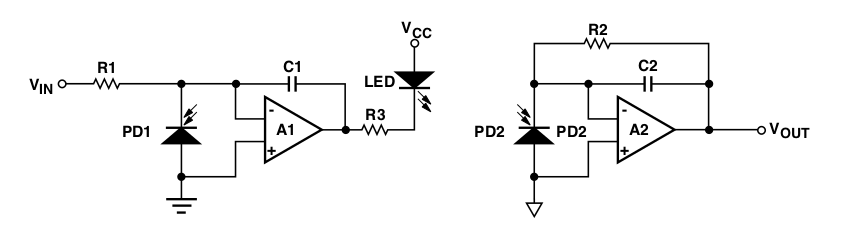
\includegraphics[scale=0.5]{Lecture/images/Analog} \\ \vspace{0cm}
				\end{center}
			
					%  BOM
					\begin{table}[h!]	
						\centering
						\begin{tabular}{|c|c|c|}
							\hline
							Part number & Description & Prix (total)\\ \hhline{|=|=|=|}
							BU7421SG-TR & Op-amp (2x) & 2\$ \\ \hline
							LOC110STR & Optocoupleur linéaire & 4.09\$ \\ \hline
							 \multicolumn{2}{|c|}{*Prix de digikey pour 1 unité }& 6.09\$ \\ \hline
						\end{tabular}
						\caption{Bill of material - Analog}
						%\label{table:BOM_Analog}
					\end{table}
						
					% Avantage // Desavantage	
					\begin{table}[h!]
					\centering
						\begin{tabular}{|c|c|}
							\hline
							Avantage & Désavantage\\ \hhline{|=|=|}
							Peu de composantes & Précision de +/- 1\% \\ \hline
							Robuste & L'optocoupleur linéaire est gros (SOIC 8)\\ \hline
							 & Consomme beaucoup de courant (10mA max)\\ \hline
						\end{tabular}
						\caption{Avantage et désavantage - Analog}
						%\label{table:Analyse_Analog}
					\end{table} 
					
				% Conclusion
				Le circuit analogique autour de l'optocoupleur linéaire n'est pas assez précis pour être considéré comme viable pour le projet.De plus, il consomme beaucoup trop de courant pour pouvoir être toujours en marche. Il faudrait ajouter un circuit pour désactiver la lecture lorsqu'elle n'est pas utilisé. Ceci enlève l'avantage d'utiliser cette solution. 
				\newpage
				
			\subsection{Circuit digital}
				\subsubsection{Protocole de communication}
					Les ADC externes utilisent souvent les même trois interface de communication sériel : UART,I2C et SPI. Puisque nous avons un nombre limité de ces periphérique sur le microcontrôleur, nous aurons besoin d'un bus qui permet d'avoir un maximum d'ADC. Il nous reste donc le choix entre le I2C et le SPI. Le SPI demanderais d'avoir un circuit d'isolation considérablement plus gros et dispendieux que le I2C. Le SPI à deux fils de plus que le I2C ( 1 pour le data et 1 pour choisir le "slave"). \\
					Le protocol choisis est le I2C et le circuit d'isolation est le ISO1541DR. Malheureusement, le circuit consomme un petit peu moins de 5mA. Nous devrons donc avoir une alimentation qui permettra de désactiver l'alimentation du côté du modules lorsque le système ne sera pas en marche.
					
				\subsubsection{Lecture d'un voltage de référence}
					La première solution envisagé étaient de lire un voltage de référence avec le ADC. Puisqu'on connait la tension à l'entrée, il est possible de déterminer la tension de l'alimentation du ADC avec la valeur de la lecture. Le ADS1013 avait été retenue puisqu'il a une alimentation de 2 à 5.5V, un quiescent current de 150$\mu$A et une résolution de 12 bits. Cependant, ce ADC a une entrée différentielle et nous aurions seulement utilisé la moitiée de la plage. Nous nous retrouverions ainsi avec uns résolution de 11 bits. En utilisant un voltage de référence de 2.048V, nous obtenerions une précision de 4.2mV lorsque le module est à 4.2V.Nous somme près de nos objectifs mais le voltage minimum pour l'alimentation de l'isolateur I2C (3V) fait en sorte que cette solution ne peut être envisagée.
					% Schema
					\begin{figure}[h]
						\centering
						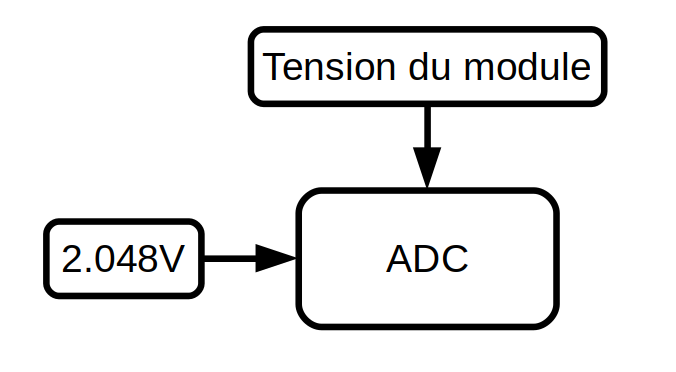
\includegraphics[scale=0.3]{./Lecture/images/Voltage_reference} \\ \vspace{0cm}
						\caption{Schéma fonctionnel : Voltage de référence }
						%\label{fig:schema_voltage_ref}
					\end{figure}

				\newpage
				\subsubsection{Lecture de la tension du module}
					Pour pouvoir mesurer la tension du module, l'alimentation du ADC doit être au dessus du voltage maximal du module plus une marge de sécurité. De plus, il est plus intéressant d'utiliser un ADC "single ended" ou "pseudo differential" pour avoir accès à toute la plage. Il est donc nécessaire d'avoir un "boost" pour amener la tension d'alimentation à 5V. Cette tension va alimenter le circuit d'isolation I2C. Un régulateur linéaire sera nécessaire pour alimenter le ADC afin d'avoir un minimum de bruit dans les lecture. Un "boost" avec l'option "shutdown" sera utilisé pour que le circuit ne vide pas les batteries lorsque le "battery pack" est entreposé. Un premier ADC, le MCP3221A5T avait été selectionné mais il fut rejeté puisqu'il est impossible de changer l'adresse du IC (elle doit être changé par la compagnie). En ce moment, les pièces envisagées sont :
					
					%  BOM
					\begin{table}[H]
						\centering
						\begin{tabular}{|c|c|c|}
							\hline
							Part number & Description & Prix (total) \\ \hhline {|=|=|=|}
							ADC121C021CIMM/NOPB & ADC 12 bit I2C & 4.3\$ \\ \hline
							AP2202K-ADJTRG1 & LDO & 0.63\$ \\ \hline
							AP3015KTR-G1 & Boost & 1.1\$ \\ \hline
							ISO1541DR & Isolation I2C & 6.67\$ \\
							   ou 	  & ou & ou \\
							SI8602AC-B-IS & Isolation I2C & 4.62 \$ \\ \hline
							LTV-816S & Optocoupleur (boost shutdown) & 0.61\$ \\ \hline
							\multicolumn{2}{|c|}{ }& 13.31 ou 11.31\$ \\ \hline
							\multicolumn{3}{r}{ } Prix de digikey pour 1 unité \\ 
						\end{tabular} \\ \vspace{0cm} 
						\caption{Bill of material - Digital}
						%\label{table:BOM_Digital}
					\end{table}
				% Schema
				\begin{figure}[h]
					\centering
					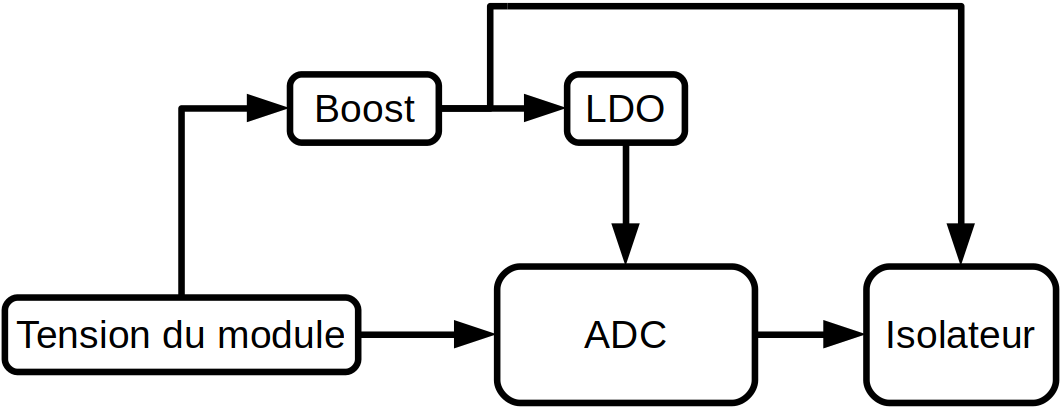
\includegraphics[scale=0.3]{./Lecture/images/Tension_module} \\ \vspace{0cm}
					\caption{Schéma fonctionnel : Lecture de la tension du module}
					%\label{fig:schema_tension_module}
				\end{figure}
			
				Un ADC secondaire (MCP3021) pourrait être connecté en parallèle avec le ADC primaire (ADC121C021CIMM/NOPB).
			
			Note : Mettre un mosfet comme protection de polariter inverse, voir pour mettre la gate sur la pin SHDN du boost pour eviter qu'il y ait un tension sur l'entrée de l'ADC lorsqu'il n'est pas alimenté.

%===== Balancement =====	
	\subsection*{Stratégies de balancement}
\paragraph*{}
Pour égaliser les tensions, le courant de recharge des modules qui ont atteint le voltage maximum peut être dissipé ou envoyé vers les modules qui ont un état de charge inférieur. 

\subsubsection*{Balancement dissipatif au voltage maximum des modules ("Top balancing")}
\paragraph*{}
Le balancement dissipatif à l'avantage d'être plus compacte, plus facile à concevoir et moins dispendieux. Le courant de recharge doit cependant pouvoir être réduit pour ne pas être plus haut que le courant de balancement. Cette technique ne permet pas de balancer avec de grand courant puisque la chaleur dégagée par la résistance et le MOSFET dégagerait trop de chaleur, ce qui peut causer une erreur de température élevée. La sensibilité du MOSFET et sa défaillance en court-circuit  font en sorte que cette méthode n'est pas très robuste. Un MOSFET en court-circuit ne déclenche aucune erreur et il peut être long avant de détecter qu'un module se vide plus rapidement que les autres. Cette erreur a le potentiel de briser la batterie dans le cas ou aucune action externe n'est prise et que le module atteint une tension en dessous du seuil minimum.

\paragraph*{}
Pour remédier à ce problème, un MOSFET contrôlé par un comparateur est mis en série avec le circuit de balancement. Cette redondance permet de couper le circuit dans lorsque la tension du module n'est pas dans la plage où il peut être balancé. Cette protection est indépendante et matérielle, elle est tout aussi efficace dans le cas où le MOSFET contrôlé par le PWM est en court-circuit ou si l'erreur provient du microcontrôleur qui envoie un PWM alors qu'il ne devrait pas.

\begin{figure}[H]
	\begin{minipage}{0.5\textwidth}
		\centering
		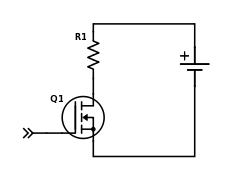
\includegraphics[scale=0.9]{Images/Dissipative_balancing.png}
		\caption{Schéma fonctionnel du balancement dissipatif}
		\label{fig:bal_dis}
	\end{minipage}
	\hfill
	\begin{minipage}{0.45\textwidth}
		\centering
		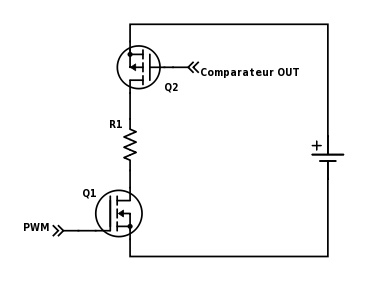
\includegraphics[scale=0.6]{Images/Dissipative_bal_comp.png}
		\caption{Schéma fonctionnel du balancement dissipatif avec redondance}
		\label{fig:bal_dis_comp}
	\end{minipage}	
\end{figure}

\subsubsection*{Balancement actif}
\paragraph*{}
Le balancement actif permet non seulement d'amener l'état de charge à 100\%, mais aussi de l'amener à 0\%. Les modules qui ont une capacité supérieure peuvent transmettre l'énergie excédentaire aux modules avec une plus petite capacité. L'utilisation de la batterie est ainsi optimisée. Plusieurs topologies existent pour transférer l'énergie telles que des capacitances commutées, deux matrices qui connectent deux différents modules sur un convertisseur DC-DC, l'utilisation d'une inductance couplée pour faire un "Flyback" et plusieurs autres variantes. 

\paragraph*{}
L'utilisation d'un convertisseur DC-DC "Flyback", avec le primaire aux bornes de chaque module et le secondaire aux bornes de la batterie, est la topologie qui s'intègre le mieux pour son nombre de composantes limitées et sa simplicité d'utilisation. Le balancement actif est surtout utilisé pour des batteries qui ont des modules avec des performances très inégales et/ou des batteries qui ont une très grande durée de vie. Cette solution est plus robuste, puisqu'il suffit d'un fusible en série avec le bobinage primaire pour protéger la batterie d'une défaillance du MOSFET. Le courant de balancement peut aussi être beaucoup plus élevé étant donné qu'il n'y a pas beaucoup de perte.

\subsubsection*{Choix final}
\paragraph*{}
Le balancement dissipatif est la stratégie qui concorde le mieux aux besoins d'Éclipse X. La grosseur des transformateurs, l'ajout des fils pour connecter les bobinages secondaires, le manque de temps pour implémenter la solution et le faible gain de performance du balancement actif rendent cette solution impossible à utiliser pour le projet. La batterie d'Éclipse a seulement une durée de vie utile de 4 semaines en plus d'être construite avec des modules caractérisés qui ont des performances très semblables. Le balancement actif n'a pas de grande valeur ajoutée par rapport au balancement dissipatif.

\newpage


%===== Detection des fautes =====
	
%===== Detection des fautes =====
\section{Détection des fautes}
	\subsection{Surcharge}
	
	\subsection{Décharge excessive}
	
	\subsection{Courant excessif}
	
	\subsection{Température}
	
	\subsection{Déconnection d'une ou plusieurs cellules}
		Une ou plusieurs cellules dans le module se deconnecte. La lecture de tension peut autant etre sur la cellule deconnecte ou non.
	\subsection{}
	
	\subsection{}
	
	\subsection{}
	
	\subsection{}
	
	\subsection{}
	
	\subsection{}
	



\end{document}
\makeatother


